\chapter{Математическая модель БОЭП как объекта управления} \label{ch:ch3}

Оптико-электронный прибор (ОЭП) вертолетного базирования имеет тепловизионный и телевизионный каналы, лазерный дальномер. Кроме того, на борту устанавливают оптико-электронную систему постановки помех (СОЭП).  Управление направлением линии визирования осуществляется перемещением всего оптико-электронного блока. Для ОЭП и СОЭП конструктивно оптико-электронный блок представляет собой блок, в котором размещены оптические приборы, вращающийся по углу места внутри вилки, вращающейся по углу азимута 
(рисунок~\ref{fig:device}, кинематическая схема на рисунке~\ref{fig:kinematic}). 
На осях вращения размещены моментные двигатели и датчики углов. ОЭП установлен в носовой части вертолета, СОЭП устанавливается в хвостовой части и на балках 
(рисунок~\ref{fig:helicopter}).

При проектировании ОЭП и СОЭП возникли задачи построения адекватной математической модели, синтеза системы управления направлением линии визирования и построения компьютерной имитационной модели ОЭП и СОЭП. Решение этих задач является продолжением работ [3/15-18]. Математическая модель строится на основе применения уравнений Лагранжа II-го рода с использованием смешанного метода Жильбера. Разработаны алгоритмы управления, обеспечивающие требуемые точностные и динамические характеристики СОЭП для режима слежения и наведения. Исследование динамических свойств СОЭП проводится с использованием компьютерной имитационной модели. Использование метода математического моделирования при проектировании бортовых СОЭП позволяет обеспечить достижение заложенных технических требований по параметрам системы, сократить сроки разработки, настройки и испытаний изделия. Компьютерная имитационная модель верифицирована по результатам настройки опытного образца.

\begin{landscape}
\section{Принципиальная схема} \label{ch:ch3/sect1}

\begin{figure}[ht]
	\centering
	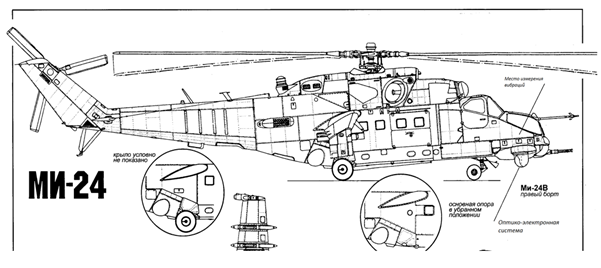
\includegraphics[width=0.9\linewidth]{img-15} 
	\caption{Принципиальная схема расположения на борту}
	\label{fig:helicopter}
\end{figure}

\begin{figure}[ht]
	\centering
	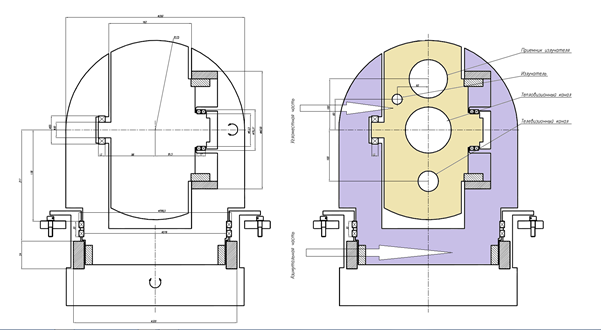
\includegraphics[width=0.9\linewidth]{img-16} 
	\caption{Общий вид изделия}
	\label{fig:device}
\end{figure}
\end{landscape}

\section{Механическая модель} \label{ch:ch3/sect2}

Исходя из анализа конструкции ОЭП для управления линией визирования оптико-электронного блока – объекта управления (ОУ) и движения вертолета (ЛА), на котором он установлен, приняты основные допущения, выбраны системы координат и определены исходные данные, необходимые для построения математической модели. ОУ.

\begin{figure}[ht]
	\centering
	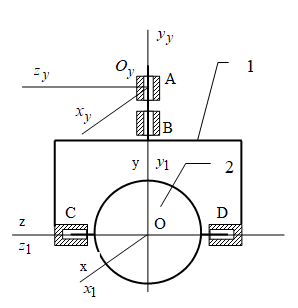
\includegraphics[]{img-17} 
	\caption{Кинематическая схема}
	\label{fig:kinematic}
\end{figure}

\subsection{Основные допущения, системы координат} \label{sec:ch3/sec3}

\begin{enumerate}
	\item ОУ моделируется двумя абсолютно твердыми телами:
	\begin{itemize}
		\item 1–е тело объединяет все элементы, вращающиеся по углу азимута вокруг оси АВ (рисунок \ref{fig:kinematic}) в неограниченном диапазоне (более $360_0$). Тело 1 (вилка) совершает вращательное движение вокруг оси АВ под действием вращающего момента, создаваемого моментным двигателем.
		\item 2–е тело (оптико-электронный блок) объединяет все элементы, вращающиеся по углу места вокруг оси CD (рисунок \ref{fig:device}). Тело 2 (оптико-электронный блок) вращается относительно тела 1 вокруг оси CD под действием вращающего момента, создаваемого другим моментным двигателем.
	\end{itemize}
	\item Ось вращения 2-го тела перпендикулярна оси вращения 1-го тела и пересекается с ней: $AB\perp CD$, т.$O \in AB$, т.$O \in CD$
	\item Инерциальная система координат, система координат связанная с вертолетом (ЛА) и установочная система координат выбраны в соответствии с принципиальной схемой расположения на борту (рисунок \ref{fig:helicopter}). Их положение и кинематические характеристики  определены выражениями (3.1)-(3.14).
	\item Система координат $O_{x_1y_1z_1}$ (Рисунок \ref{fig:coord/3.4}) жестко связана с 1-м телом. 
	\begin{figure}[ht]
		\centering
		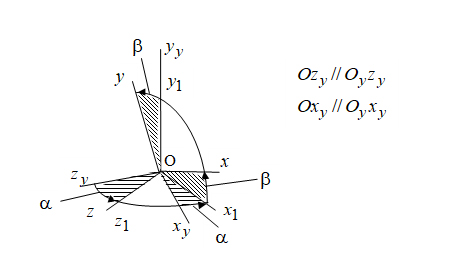
\includegraphics[]{img-18} 
		\caption{Кинематическая схема}
		\label{fig:coord/3.4}
	\end{figure}

	Ось $O_{y_1}$ направлена по оси вращения АВ, ось $O_{z_1}$ направлена по оси вращения CD, ось $O_{x_1}$ дополняет указанные оси до правой системы координат. Точка O находится на пересечении осей АВ и CD. Положение точки О в установочной системе координат определяется радиусом-вектором
	\item Оси
	\item Движение ЛА происходит в однородном поле силы тяжести.
\end{enumerate}


\subsection{Геометрия масс} \label{sec:ch3/sec4}

По рабочим чертежам в среде Solid Works получены массовые характеристики ОУ. Их обозначения и величины приведены в таблице ниже (Таблица 3.1).


\section{Составление уравнений динамической модели ОУ} \label{ch:ch3/sect5}


\subsection{Вычисление кинетической энергии} \label{sec:ch3/sec6}

\subsection{Вычисление обобщенных сил} \label{sec:ch3/sec7}

\subsection{Составление уравнений динамической модели ОУ} \label{sec:ch3/sec8}


\section{Модель привода} \label{ch:ch3/sect9}

\section{Линеаризованная система} \label{ch:ch3/sect10}

\section{Выводы по главе} \label{ch:ch3/sect11}


Некоторый текст.

\clearpage